\newthought{\textbf{Nurul Aflah - 2020903430036 - TRKJ 3B}}

\newday{\textbf{1-2 Desember 2022}-instalasi dan konfigurasi apache hadoop}
\begin{enumerate}
\item Kendala dan Solusi
\newline praktikum instalasi apache hadoop tidak ada kendala, tetapi pada konfigurasi apache hadoop terkendala pada saat perintah jps, hasil yang muncul hanya 2jps, solusinya yaitu kembali pada langkah ssh, untuk menampilkan jps harus berada pada /usr/local/etc/hadoop.

\item Kesimpulan
\newline berhasil melakukan instalasi dan konfigurasi apache hadoop.

\begin{figure} [!ht]
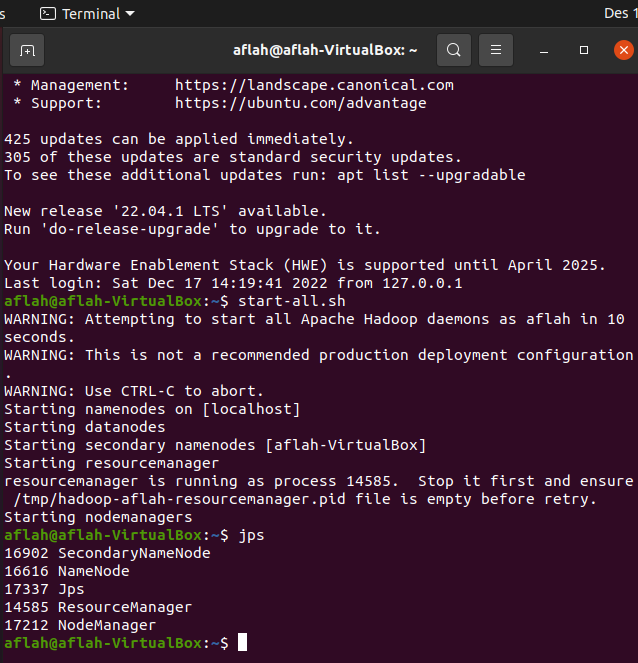
\includegraphics[width=\textwidth] {NurulAflah/jps}
\caption{hasil dari jps}
\label{gam:jps}
\end{figure}

\begin{figure} [!ht]
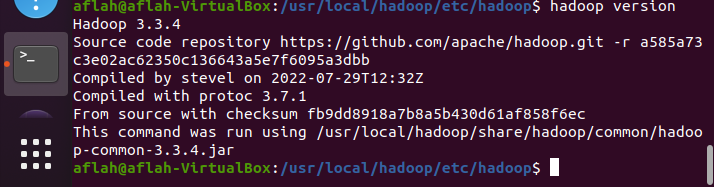
\includegraphics[width=\textwidth] {NurulAflah/hasil dari hadoop version}
\caption{hasil dari hadoop version}
\label{gam:hasil dari hadoop version}
\end{figure}

\begin{figure} [!ht]
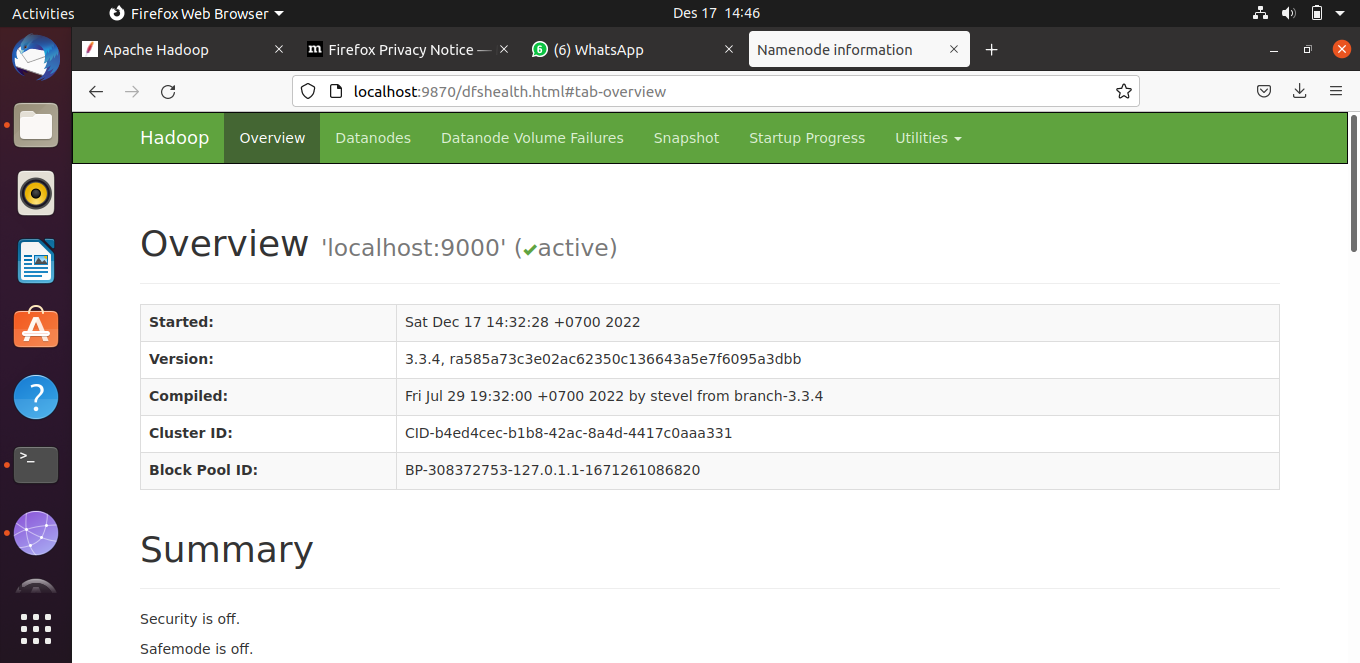
\includegraphics[width=\textwidth] {NurulAflah/localhost 9870}
\caption{hasil dari localhoost}
\label{gam:localhost 9870}
\end{figure}

\begin{figure} [!ht]
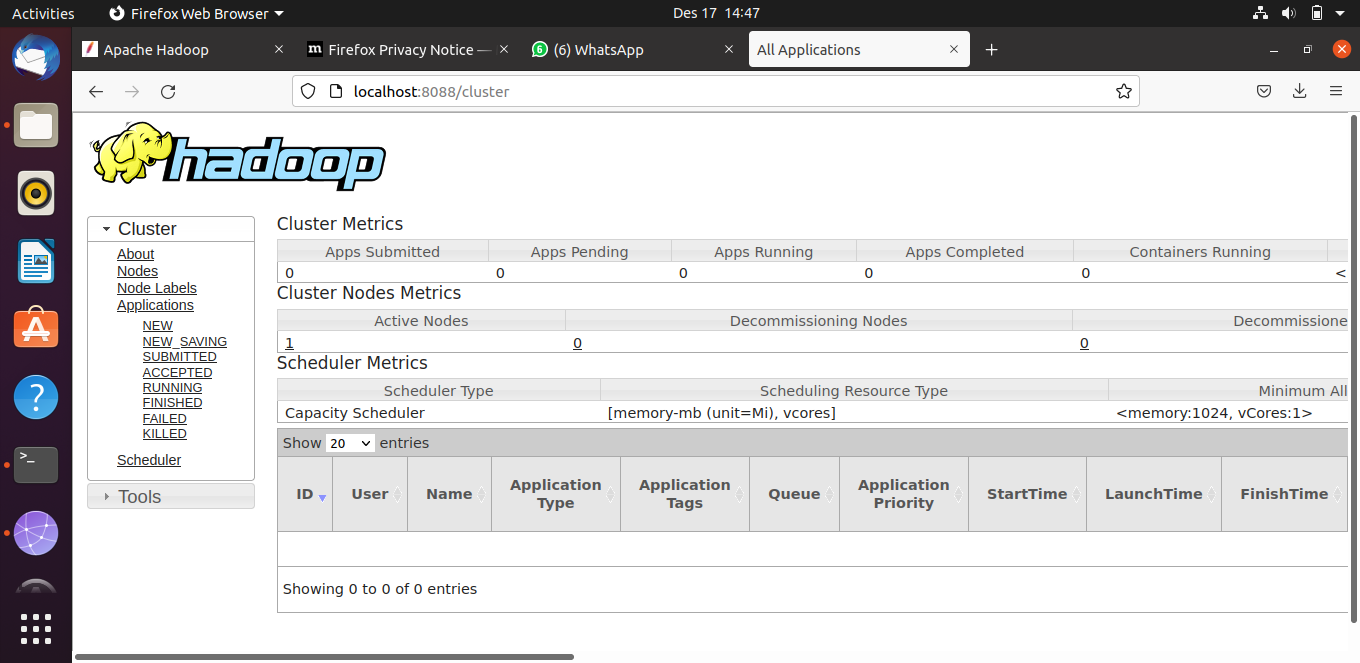
\includegraphics[width=\textwidth] {NurulAflah/local host 8088}
\caption{hasil dari localhoost}
\label{gam:local host 8088}
\end{figure}
\end{enumerate}


\newday{\textbf{8 Desember 2022}}
\begin{enumerate}
\item Kendala dan Solusi
% jelaskan kendala dan penyebab yang dialami saat mengikuti praktikum serta solusi atau langkah-langkah yang telah dilakukan

\item Kesimpulan
% berikan kesimpulan dari praktikum yang telah dikerjkan

\end{enumerate}

\newday{\textbf{9 Desember 2022}}
\begin{enumerate}
\item Kendala dan Solusi
% jelaskan kendala dan penyebab yang dialami saat mengikuti praktikum serta solusi atau langkah-langkah yang telah dilakukan

\item Kesimpulan
% berikan kesimpulan dari praktikum yang telah dikerjkan

\end{enumerate}

\newday{\textbf{15 Desember 2022}-program wordcount bawaan hadoop}
\begin{enumerate}
\item Kendala dan Solusi
\newline tidak ada kendala pada melakukan praktikum program wordcount hadoop ini.

\item Kesimpulan
\newline berhasil melakukan praktikum ini.

\begin{figure} [!ht]
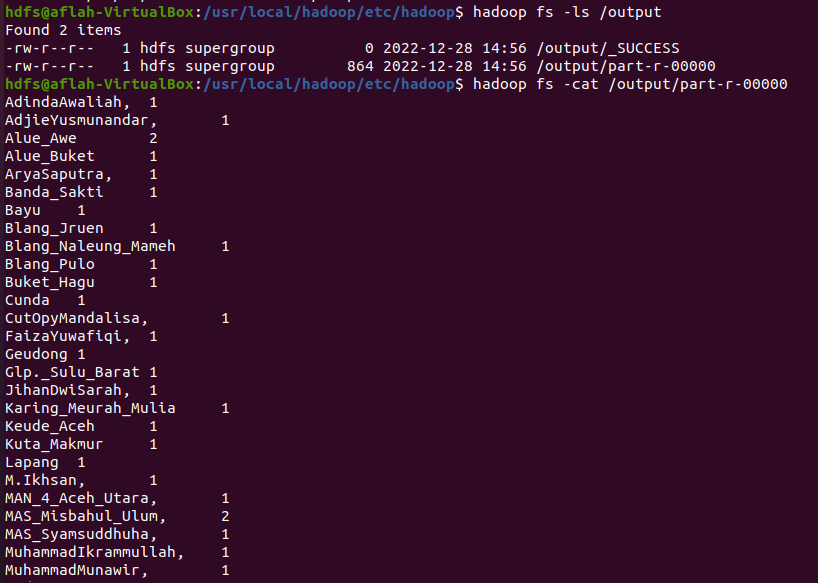
\includegraphics[width=\textwidth] {NurulAflah/6 dan 7a}
\caption{hasil dari perintah ke 6 dan 7}
\label{gam:6 dan 7a}
\end{figure}
\end{enumerate}


\newday{\textbf{16 Desember 2022}-wordcount java}
\begin{enumerate}
\item Kendala dan Solusi
\newline tidak ada kendala saat melakukan praktikum wordcuont java ini.

\item Kesimpulan
\newline berhasil melakukan praktikum ini.
\newpage
\begin{figure} [!ht]
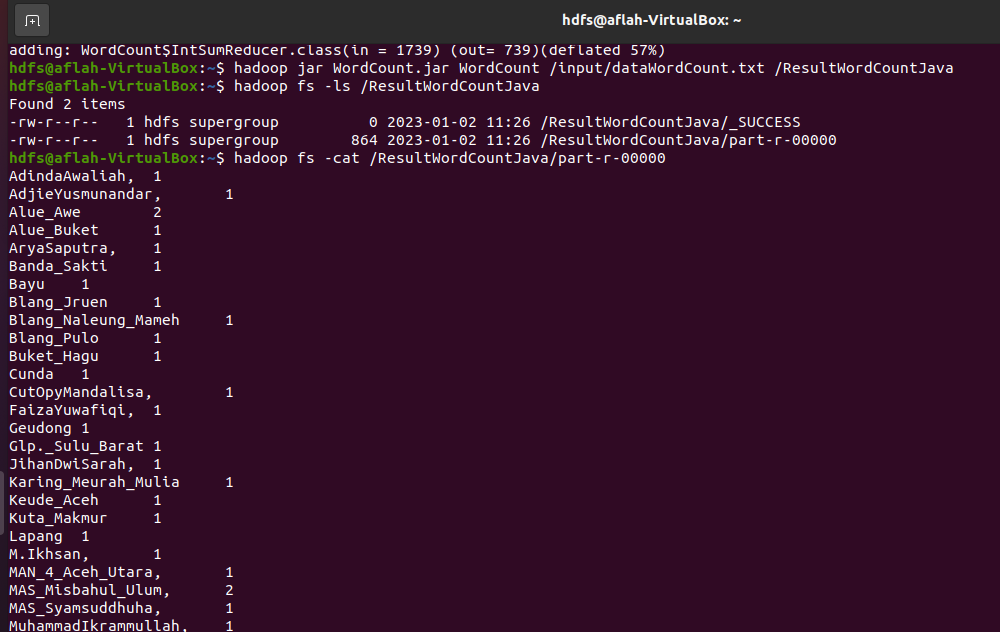
\includegraphics[width=\textwidth] {NurulAflah/9 dan 10a}
\caption{hasil dari perintah wordcount java}
\label{gam:9 dan 10a}
\end{figure}

\begin{figure} [!ht]
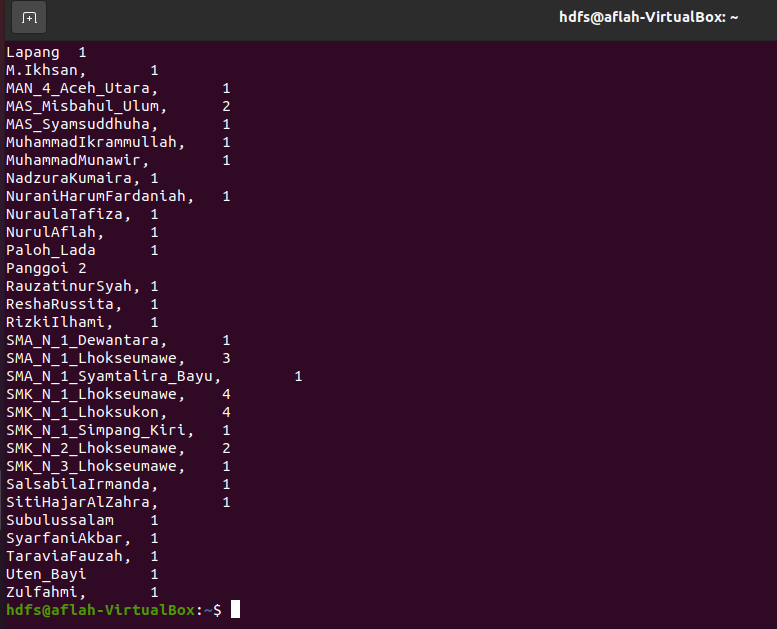
\includegraphics[width=\textwidth] {NurulAflah/10b}
\caption{hasil dari perintah wordcount java}
\label{gam:10b}
\end{figure}
\end{enumerate}

\newday{\textbf{22 Desember 2022}-instalasi apache spark}
\begin{enumerate}
\item Kendala dan Solusi
\newline tidak ada kendala saat melakukan praktikum instalasi apache spark ini.

\item Kesimpulan
\newline berhasil melakukan praktikum ini.

\begin{figure} [!ht]
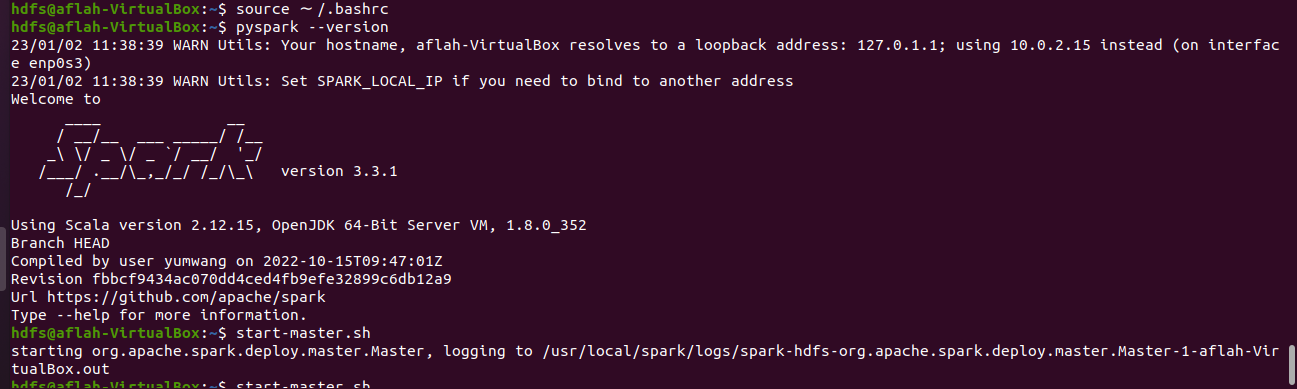
\includegraphics[width=\textwidth] {NurulAflah/instalasi py spark}
\caption{hasil dari perintah instalasi py spark}
\label{gam:instalasi py spark}
\end{figure}
\end{enumerate}


\newday{\textbf{23 Desember 2022}-program wordcount dengan python}
\begin{enumerate}
\item Kendala dan Solusi
\newline tidak ada kendala saat melakukan praktikum program wordcount dengan python ini.

\item Kesimpulan
\newline berhasil melakukan praktikum ini.
\newpage
\begin{figure} [!ht]
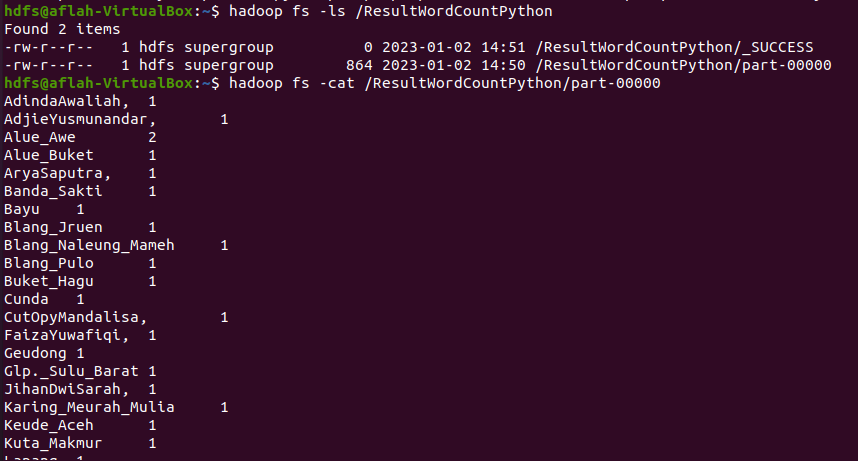
\includegraphics[width=\textwidth] {NurulAflah/hasil hadoop jar python}
\caption{hasil dari perintah wordcount python}
\label{gam:hasil hadoop jar python}
\end{figure}

\begin{figure} [!ht]
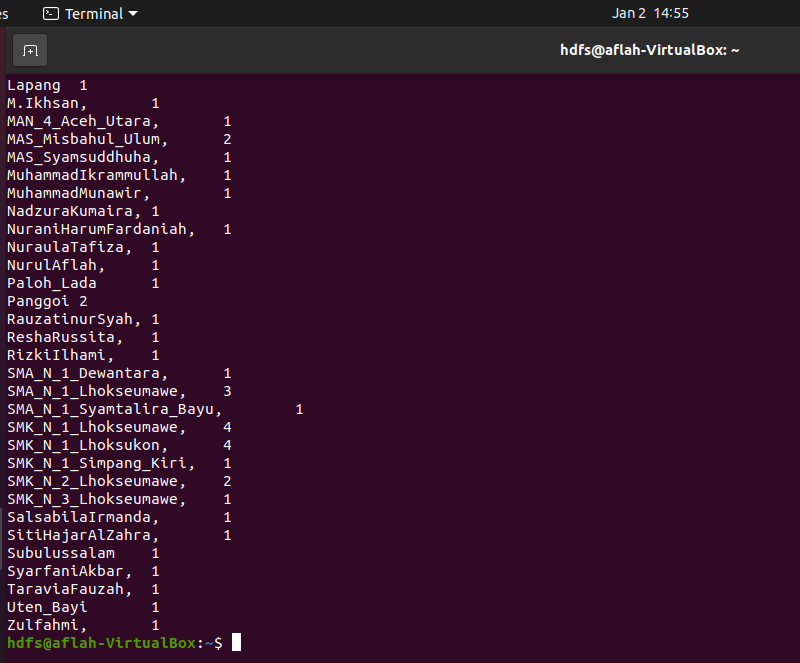
\includegraphics[width=\textwidth] {NurulAflah/hadoop jar python}
\caption{lanjutan dari perintah wordcount python}
\label{gam:hadoop jar python}
\end{figure}
\end{enumerate}

\newday{\textbf{23 Desember 2022}-program wordcount dengan py spark}
\begin{enumerate}
\item Kendala dan Solusi
\newline tidak ada kendala saat melakukan praktikum program wordcount dengan py spark ini.

\item Kesimpulan
\newline berhasil melakukan praktikum ini.
\newpage
\begin{figure} [!ht]
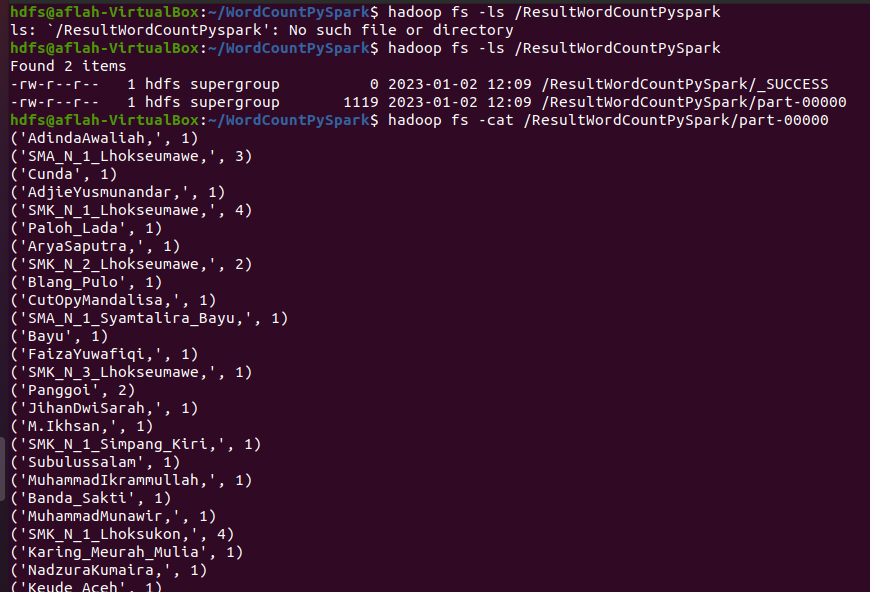
\includegraphics[width=\textwidth] {NurulAflah/hasil pyspark}
\caption{hasil dari perintah wordcount py spark}
\label{gam:hasil pyspark}
\end{figure}
\end{enumerate}


\newday{\textbf{tugas individu}-program machine learning dengan pyspark}
\begin{enumerate}
\item Kendala dan Solusi
\newline tidak ada kendala saat melakukan praktikum program machine learning dengan py spark ini.

\item Kesimpulan
\newline berhasil melakukan praktikum ini.

\begin{figure} [!ht]
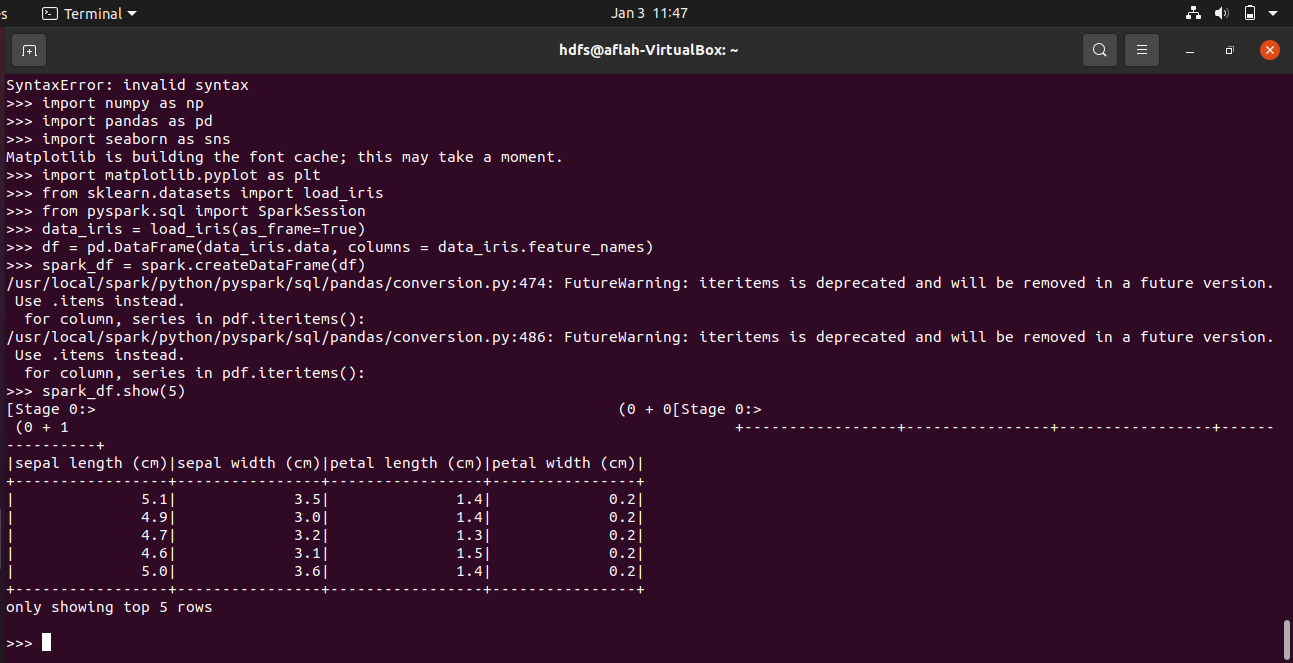
\includegraphics[width=\textwidth] {NurulAflah/hasil1 tugas individu}
\caption{hasil dari tabel pertama}
\label{gam:hasil1 tugas individu}
\end{figure}

\begin{figure} [!ht]
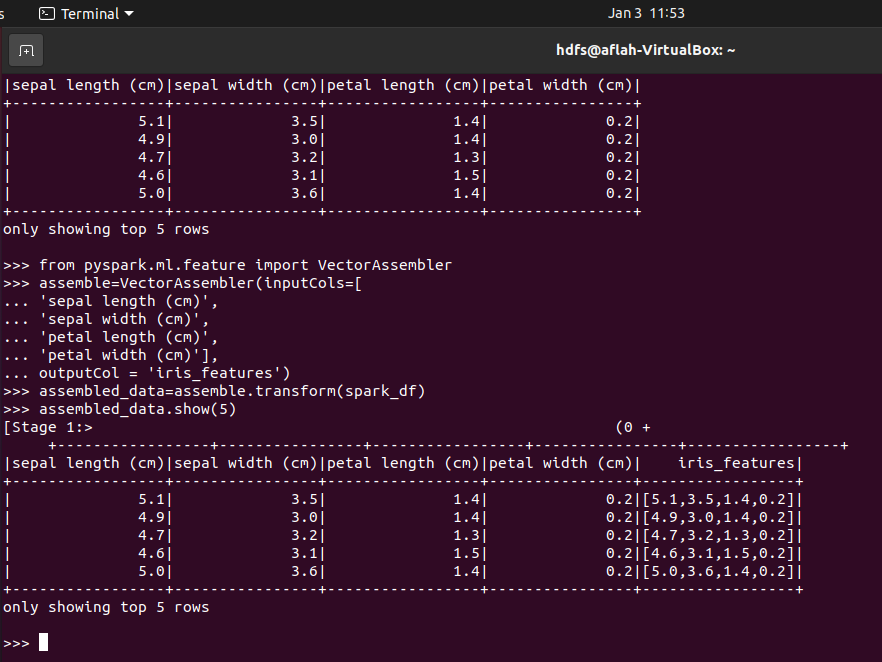
\includegraphics[width=\textwidth] {NurulAflah/hasil2 tugas individu}
\caption{hasil dari tabel kedua}
\label{gam:hasil2 tugas individu}
\end{figure}

\begin{figure} [!ht]
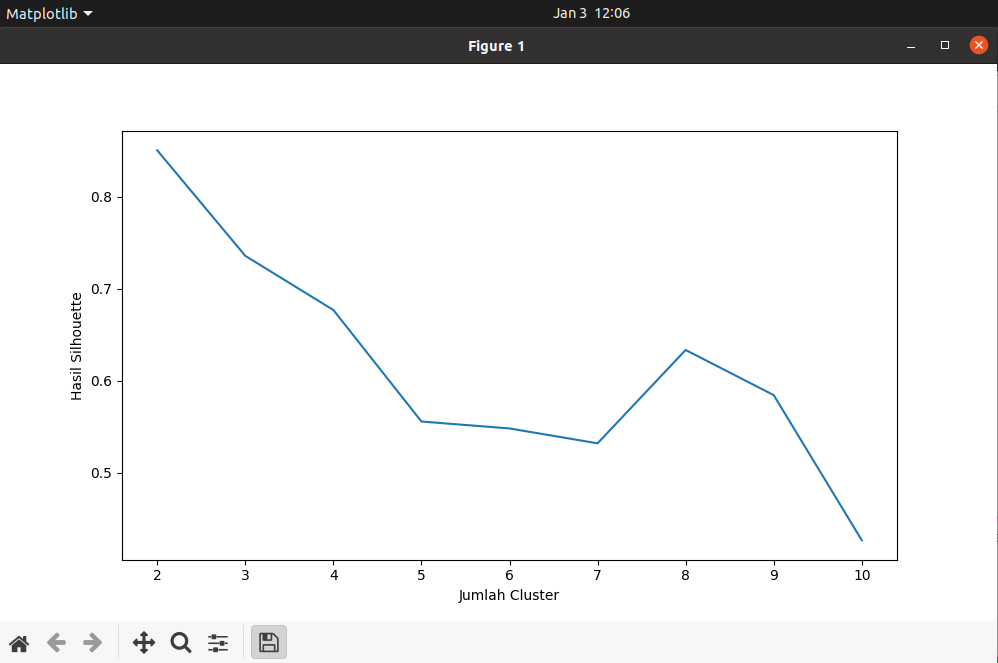
\includegraphics[width=\textwidth] {NurulAflah/grafik figure1}
\caption{hasil dari grafik pertama}
\label{gam:grafik figure1}
\end{figure}

\begin{figure} [!ht]
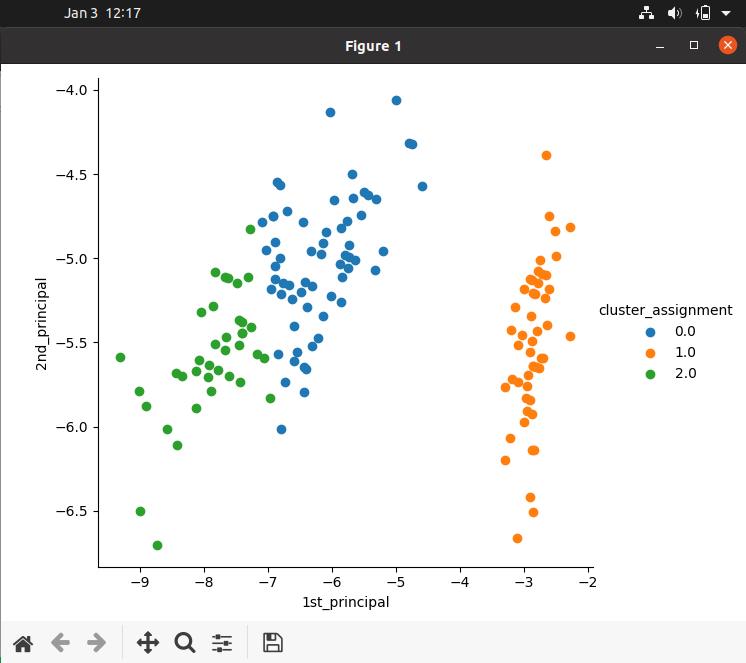
\includegraphics[width=\textwidth] {NurulAflah/grafik figure2}
\caption{hasil dari grafik kedua}
\label{gam:grafik figure2}
\end{figure}
\end{enumerate}